\documentclass[../thesis.tex]{subfiles}
\begin{document}

\chapter{Introduction}
\label{chp:introduction}

This chapter gives a short introduction to the overall research field this work addresses. After that is done the objectives and structure of this work are explained.

\section{Motivation}

With the development towards higher resource efficiency and sustainability, new materials and chemicals have to be developed to replace the fossil based ones currently in use today. With the demand of materials constantly changing and new developments needing scale-up from laboratory scale to industrial scale, the research in microfluidic reactors has gained more and more significance in recent history. These systems have the advantage of being easily customizable and having the capability of dealing with toxic or explosive materials, due to their low reaction volume. This, in addition to their easy to handle geometric dimensions, makes them great for laboratory research. When looking into such small reaction systems, the evolution of a reactions appearance in space and time is of high interest. Having a deeper knowledge can be used to further improve the reactions yield or heat transfer, in case of needed heating or cooling. An example of such an microfluidic system is shown in \autoref{fig: reactor_examp}.
\begin{figure}[htb]
	\centering
	\subfloat[\centering micro fluidic reactor]{{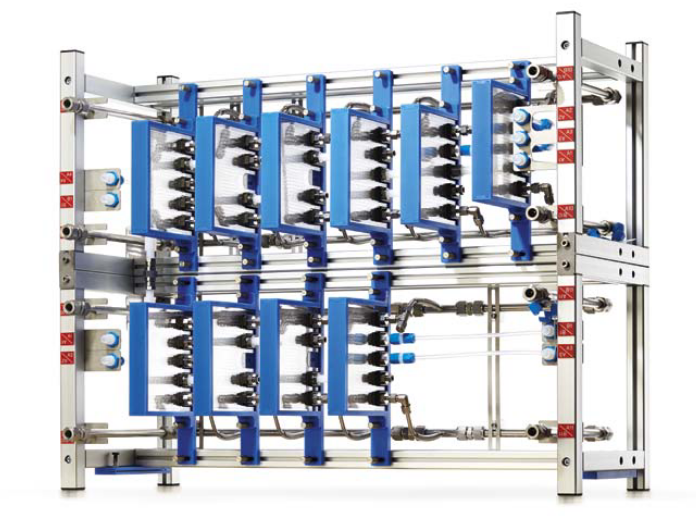
\includegraphics[scale=0.3]{reactor_example} }}%
	\qquad
	\subfloat[\centering micro flow element]{{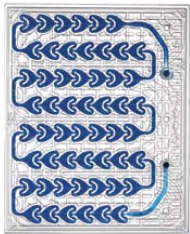
\includegraphics[scale=0.7]{reactor_element} }}%
	\caption{Microfluidic system \cite{corning}}%
	\label{fig: reactor_examp}%
\end{figure}
Customization being not challenging by placing different micro flow elements in series, the industry can quickly adapt to upcoming new research or changing market environments.

Reactions taking place under these conditions are affected by advection as a result of the moving fluid and diffusion as a result of concentration gradients. Therefore the whole moving system is called Reaction-Diffusion-Advection front or RDA.

Reaction-diffusion (RD) fronts do play a role in a large variety of natural and technical systems. From population dynamics \cite{chen2018hopf, wang2019persistence}, disease spreading \cite{kuto2017concentration, noble1974geographic, may1991infectious}, biological applications like pattern formation \cite{nakagaki1999reaction}, stability analysis in physics \cite{ebert2000front} to finance modelling in economics \cite{mastromatteo2014anomalous} and language depth modelling in linguistics \cite{abrams2003modelling}, the RD dynamics can be applied to varies different research fields. In addition to the fields already mentioned, RD with added species transport by advection, can be used to describe their distribution within different kind of reactors in the field of chemical engineering \cite{brau2020influence} or chemistry \cite{heidel1988pattern, von2013measurement}. Reaction diffusion advection fronts (RDA) can also be applied to mineralization processes \cite{schuszter2016calcium}, reactions taking place within a droplet \cite{tsuji2012chemical} or other geological processes \cite{al2019simulation} to name a few.

The foundation of reaction-diffusion-advection front research was way laid by G\'{a}lfi and R\'{a}cz \cite{galfi1988properties}, with their theoretical study on a one-dimensional (1D) case. Their predictions were then approved by simulations \cite{jiang1990simulation} and experimental observations \cite{koo1991space} in the following years. In recent times the influence of gravitation \cite{eckert2012} among other influences is of research interest. Theoretical and experimental studies which were mostly done for 2D rectilinear cases \cite{brau2020influence} were then carried out to radial geometries \cite{toth2020effects, comolli2021dynamics ,stergiou2022effects} and evolving surfaces \cite{kim2020pattern} in more recent years.
The investigations done within radial geometries for axisymmetric cases \cite{toth2020effects, comolli2021dynamics} do focus on the long term evolutions of the fronts shape and metrics. At these later stages the front has reached a final state where it's parameters do not change any more \cite{brau2020influence}.

To gain further knowledge on how the front's shapes are initially built and how the front's metrics behave at early time stages, theoretical models are needed. These models do provide a side view, otherwise not accessible by experiments with their top down point of view.
\begin{figure}[htbp]
	\centering
	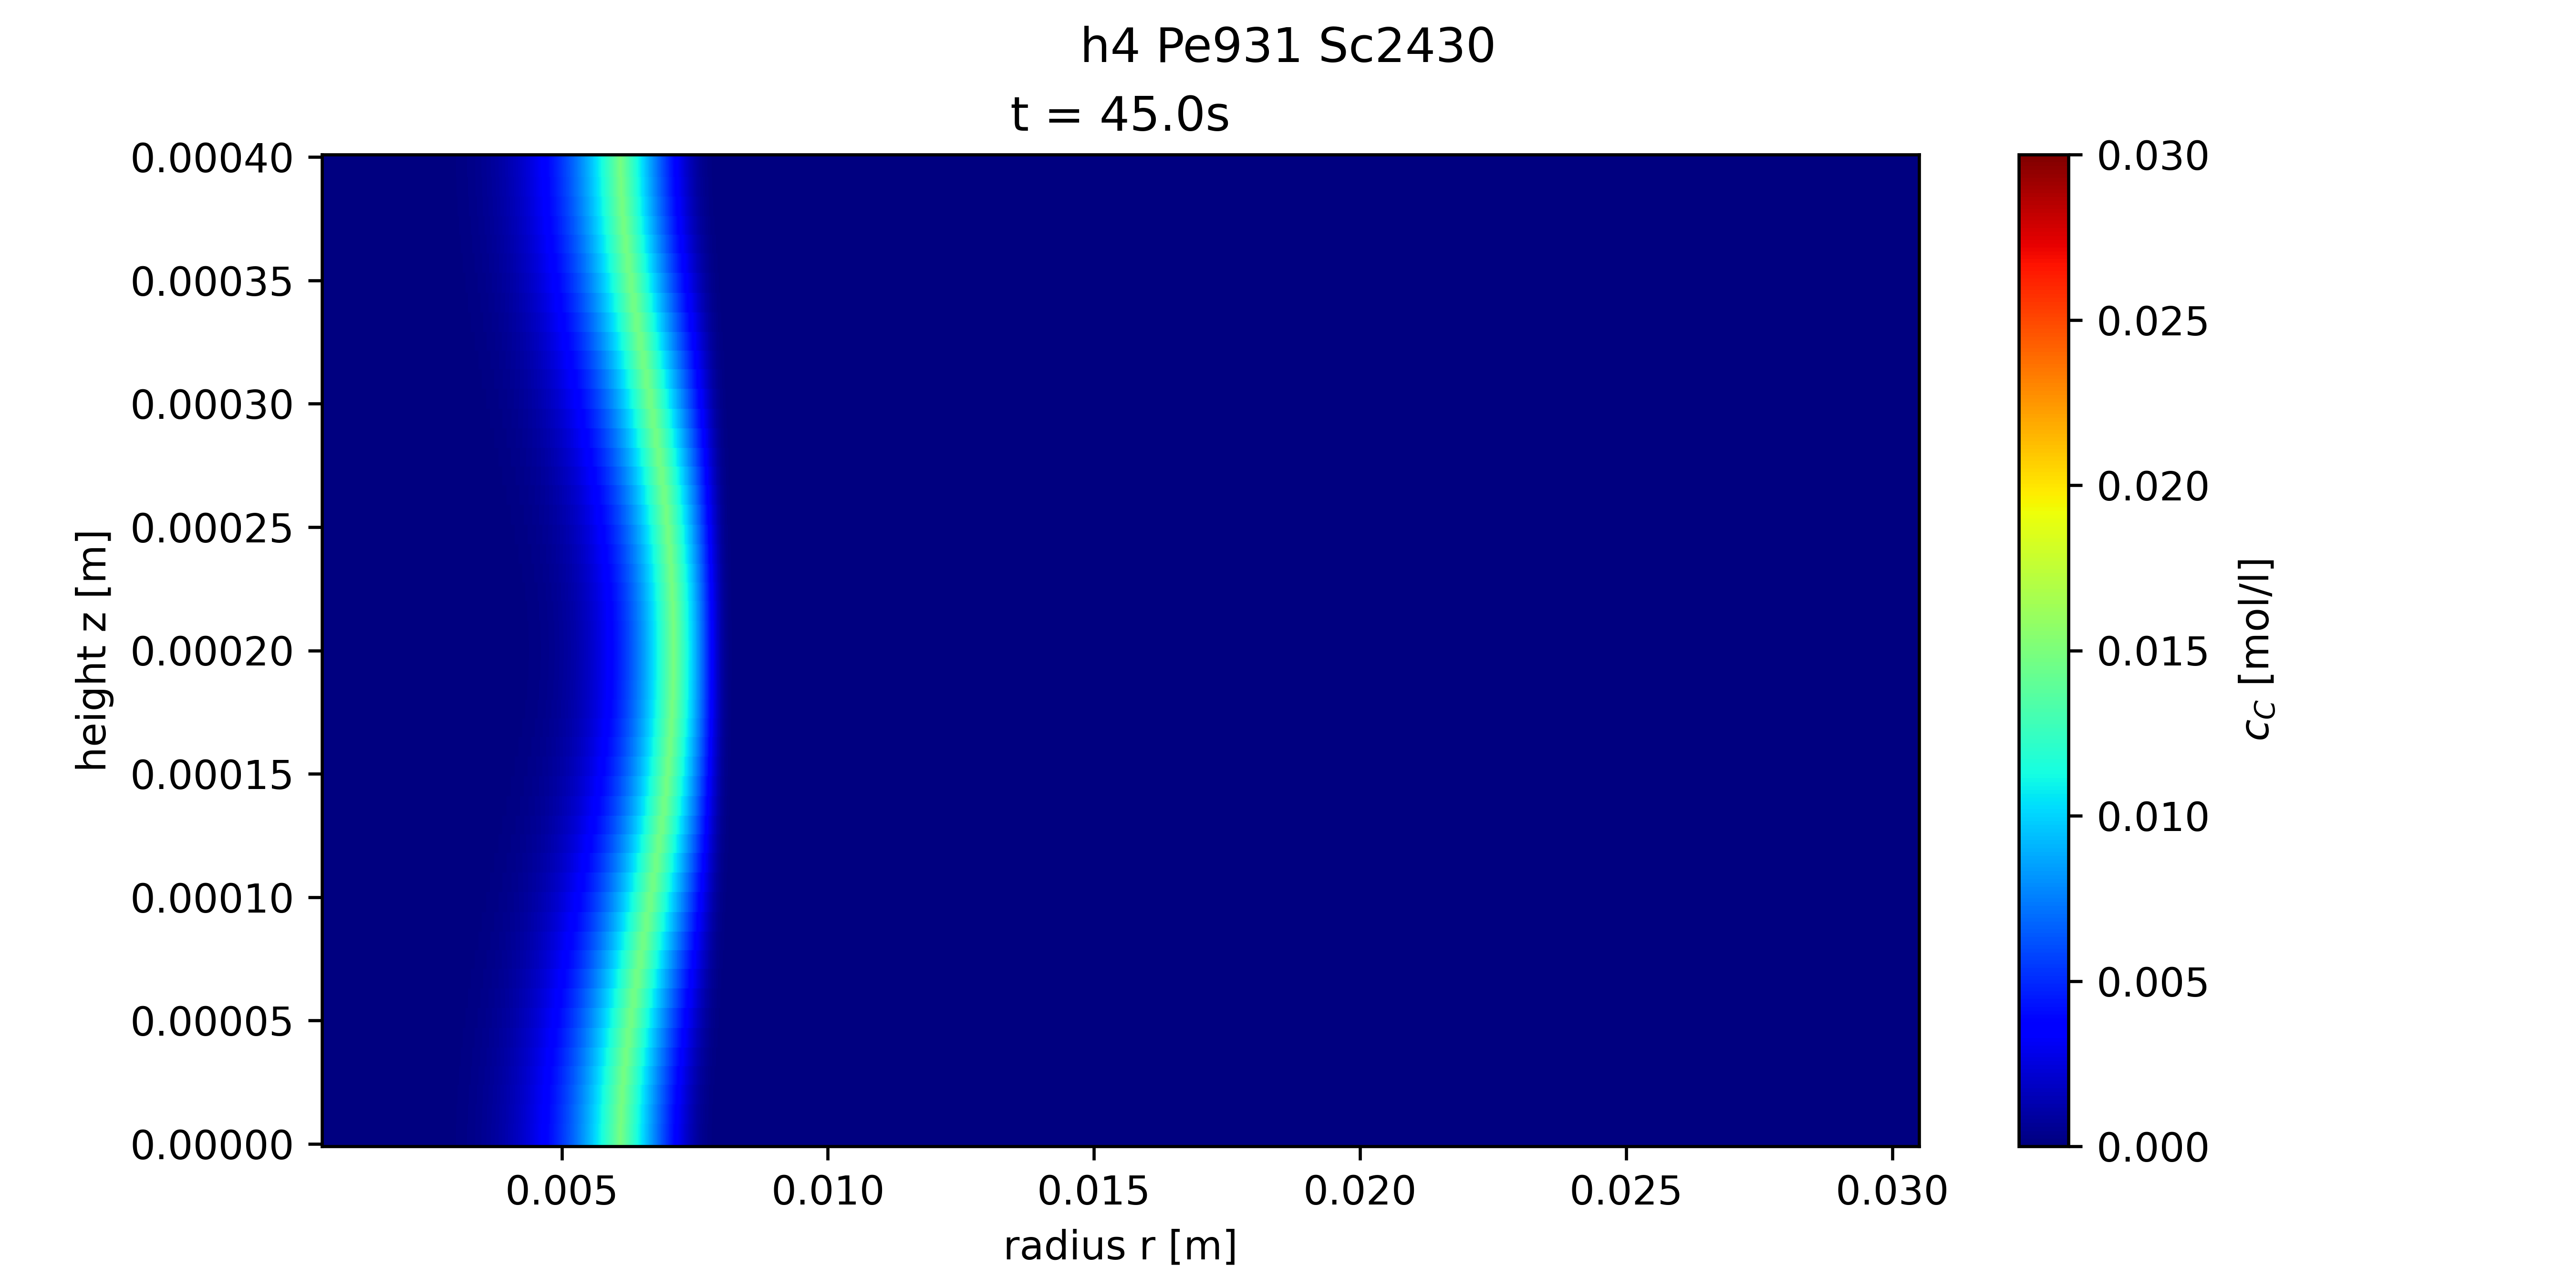
\includegraphics[width=0.8\textwidth]{front_example}
	\caption{Reaction-diffusion-advection front example}
	\label{fig: front_example}
\end{figure}
As known from previous research the fronts curvature is dependent on the system's geometry and other input values. An example of such a front appearance is shown in \autoref{fig: front_example}.

Within this work a model for the reaction-diffusion-advection system following the reaction $ A+B \rightarrow C$ is developed for a cylindrical geometry. Within this model the two initially separated species $A$ and $B$ are transported through advection and diffusion. $A$ is injected radially into $B$ from the cylinders centreline. With these conditions set, the geometry does not need to be modelled in 3D, as it is assumed to be an axisymmetric problem. Therefore a 2D approach is used.

Special interest is in the species distribution at early stages of the developing reaction front. Experiments under $0g$ conditions \cite{stergiou2022effects} have shown that gravity affects the front's shape. These effects can be seen within the schematic in \autoref{fig: 0g_example}.
\begin{figure}[htbp]
	\centering
	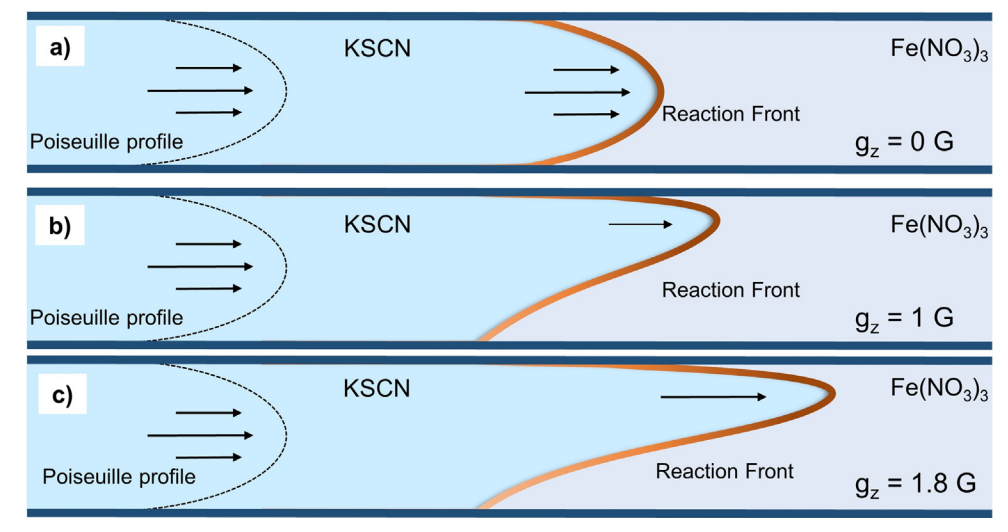
\includegraphics[width=0.8\textwidth]{0g_example}
	\caption{Schematic of gravity effects on reaction fronts \cite{stergiou2022effects}}
	\label{fig: 0g_example}
\end{figure}
Within a model gravity can be turned off, so investigations by changing geometric dimensions and other input values can be done more easily and quickly.

\section{Objectives and Report Outline}

This work aims to provide detailed insights into the early-time regime within a RDA front's development process within a radial reactor, using different input parameters. To achieve that a numerical model is created using the modelling environment \texttt{ANSYS FLUENT} \cite{manual2009ansys}. 

This work is divided into 6 chapters. The theoretical background required for modelling is given in Chapter \ref{chp:theory}. Following that the process of model creation and validation are described in Chapter \ref{chp:model}. After that results of the parametric studies are shown and discussed within Chapter \ref{chp: para_stud}. Section \ref{chp: dicus} discusses the limitations of the build model. Finally Chapter \ref{chp:out_con} summarizes the work and provides an outlook for further studies. 

\end{document}